\newpage
\section{Class \Iclass{circle}} % (fold)
\label{sec:class_circle}

\subsection{Attributes of a circle} % (fold)
\label{sub:attributes_of_a_circle}
This class is also defined by two points: on the one hand, the center and on the other hand, a point through which the circle passes.

\begin{mybox}
   Creation |C.OA = circle: new (z.O,z.A) |
\end{mybox}

\bgroup
\catcode`_=12
\small
\captionof{table}{Circle attributes.}\label{circle:att}
\begin{tabular}{lll}
\toprule
\textbf{Attributes}     & \textbf{Application} &\\
\Iattr{circle}{center}  & |z.A = C.AB.center| &\\
\Iattr{circle}{through} & |z.B = C.AB.through| &\\
\Iattr{circle}{type}    &  |C.AB.type|   &  |C.OA.type = 'circle'|\\
\Iattr{circle}{radius}  &  |C.AB.radius| &   |r = C.OA.radius | $r$ real number\\
\Iattr{circle}{north}   &  |C.AB.north|  &   |z.N = C.OA.north|\\
\Iattr{circle}{south}   &  |C.AB.south|  &    |z.S = C.OA.south| \\
\Iattr{circle}{east}    &  |C.AB.east|   &   |z.E = C.OA.east| \\
\Iattr{circle}{west}    &  |C.AB.west|   &   |z.W = C.OA.west| \\
\Iattr{circle}{opp}    &  |z.Ap = C.AB.opp|   & see (\ref{ssub:example_circle_attributes})  \\
\Iattr{circle}{ct}    &  |L = C.AB.ct|   & see (\ref{ssub:example_circle_attributes})   \\
\bottomrule %
\end{tabular}
\egroup

\subsubsection{Example: circle attributes} % (fold)
\label{ssub:example_circle_attributes}

Three attributes are used (south, west, radius).  

\begin{minipage}{0.5\textwidth}
\begin{tkzexample}[latex=0cm,small,code only]
\begin{tkzelements}
   scale = .5
   z.a   = point: new (1, 1)
   z.b   = point: new (5, 4)
   C.ab  = circle : new (z.a,z.b)
   z.s   = C.ab.south
   z.w   = C.ab.west
   r     = C.ab.radius
   z.c   = C.ab.opp
   z.r,z.t = get_points (C.ab.ct : ortho_from (z.b))
\end{tkzelements}
\begin{tikzpicture}
\tkzGetNodes
\tkzDrawPoints(a,b,c,s,w)
\tkzLabelPoints(a,b,c,s,w)
\tkzDrawCircle(a,b)
\tkzDrawSegments(a,b r,t b,c)
\tkzLabelSegment[sloped](a,b){ab = \tkzUseLua{r}}
\end{tikzpicture}
\end{tkzexample}
\end{minipage}
\begin{minipage}{0.5\textwidth}
\begin{tkzelements}
   scale = .5
   z.a = point: new (1, 1)
   z.b = point: new (5, 4)
   C.ab = circle : new (z.a,z.b)
   z.s = C.ab.south
   z.w = C.ab.west
   r   = C.ab.radius
   z.c   = C.ab.opp
   z.r,z.t = get_points (C.ab.ct : ortho_from (z.b))
\end{tkzelements}
\hspace*{\fill}
\begin{tikzpicture}
\tkzGetNodes
\tkzDrawPoints(a,b,c,s,w)
\tkzLabelPoints(a,b,c,s,w)
\tkzDrawCircle(a,b)
\tkzDrawSegments(a,b r,t b,c)
\tkzLabelSegment[sloped](a,b){ab = \tkzUseLua{r}}
\end{tikzpicture}
\hspace*{\fill}
\end{minipage}
% subsubsection example_circle_attributes (end)
% subsection attributes_of_a_circle (end)

\newpage
\subsection{Methods of the class circle} % (fold)
\label{sub:methods_of_the_class_circle}
\bgroup
\catcode`_=12
\small
\captionof{table}{Circle methods.}\label{circle:met}
\begin{tabular}{lll}
\toprule
\textbf{Methods} & \textbf{Comments}   & \\
\midrule   \\
\Imeth{circle}{new(O,A)} & |C.OA = circle : new (z.O,z.A)| & circle  center $O$ through $A$\\
\Imeth{circle}{radius(O,r)} & |C.OA = circle : radius (z.O,2)| & circle  center $O$ radius =2 cm\\
\Imeth{circle}{diameter(A,B)} & |C.OA = circle :diameter(z.A,z.B)| & circle diameter $[AB]$  \\
\midrule 
 \textbf{Points} &&\\
\midrule 
\Imeth{circle}{antipode (pt)} & |z.C = C.OA: antipode (z.B)| &    $[BC]$ is a diameter   \\
\Imeth{circle}{inversion (pt)} & |z.Bp = C.AC: inversion (z.B)|&\\
\Imeth{circle}{midarc (pt,pt)} & |z.D = C.AB: midarc (z.B,z.C)|& $D$ is the midarc of $\widearc{BC}$\\
\Imeth{circle}{point (r)} & |z.E = C.AB: point (0.25)|& |r| between 0 and 1\\
\Imeth{circle}{random\_pt(lower, upper)} & &\\
\Imeth{circle}{internal\_similitude (C)}  &  |z.I  = C.one : internal_similitude (C.two)| &\\
\Imeth{circle}{external\_similitude (C)} &    |z.J  = C.one : external_similitude (C.two)|  & \\ 
\Imeth{circle}{radical\_center (C1<,C2>)} &  or only (C1) & see \ref{sub:radical_center}   \\
\midrule 
 \textbf{Lines} & & \\
\midrule 
\Imeth{circle}{radical\_axis (C)} &  see ( \ref{sub:d_alembert_2} ; \ref{sub:radical_axis_v1} ; \ref{sub:radical_axis_v2} ; \ref{sub:radical_axis_v3} ; \ref{sub:radical_axis_v4})& \\
\Imeth{circle}{tangent\_at (pt)} & |z.P = C.OA: tangent_at (z.M)| & see (\ref{ssub:lemoine} ; \ref{ssub:example_combination_of_methods})\\
\Imeth{circle}{tangent\_from (pt)}& |z.M,z.N = C.OA: tangent_from (z.P)| & see (\ref{tangent_from})\\
\Imeth{circle}{inversion (line)} & |L or C = C.AC: inversion (L.EF)|& see (\ref{ssub:inversion_line})\\
\Imeth{circle}{common\_tangent (C)} & |z.a,z.b = C.AC: common_tangent (C.EF)|& see  (\ref{sub:common_tangent} ; \ref{sub:common_tangent_orthogonality})\\
\midrule 
 \textbf{Circles}& &\\
\midrule 
\Imeth{circle}{orthogonal\_from (pt)}  & |C = C.OA: orthogonal_from (z.P)|  & see (\ref{ssub:altshiller} ; \ref{sub:common_tangent_orthogonality} ; \ref{sub:orthogonal_circles_v1} ; \ref{sub:pencil_v1}) \\
\Imeth{circle}{orthogonal\_through (pta,ptb)}  & |C = C.OA: orthogonal_through (z.z1,z.z2)| & see (\ref{sub:orthogonal_circle_through})\\
\Imeth{circle}{inversion (...)} & | C.AC: inversion (pt, pts, L or C )|& see \ref{ssub:inversion}, \ref{ssub:inversion_point},  \ref{ssub:inversion_line},  \ref{ssub:inversion_circle}\\
\Imeth{circle}{midcircle (C)}  & |C.inv = C.OA: midcircle (C.EF)|  & see \ref{ssub:midcircle} \\
\Imeth{circle}{radical\_circle (C1<,C2>)} & or only (C1) & see \ref{sub:radical_circle}\\
\midrule 
 \textbf{Miscellaneous} &&\\
\midrule 
\Imeth{circle}{power (pt)}     &|p = C.OA: power (z.M)| &   see (\ref{sub:power_v1} ; \ref{sub:power_v2} ; \ref{sub:apollonius_circle_v1_with_inversion})  \\
\Imeth{circle}{in\_out (pt)} & |C.OA : in_out (z.M)| & see (\ref{sub:in_out_for_circle_and_disk})  \\
\Imeth{circle}{in\_out\_disk (pt)} & |C.OA : in_out_disk (z.M)| & see (\ref{sub:in_out_for_circle_and_disk})  \\
\Imeth{circle}{draw ()} & for further use &\\
\Imeth{circle}{circles\_position (C1)} & result = string &see (\ref{sub:circles_position}) \\
\bottomrule 
\end{tabular}
\egroup
% subsection methods_circle (end)

\subsubsection{Altshiller} % (fold)
\label{ssub:altshiller}

\begin{minipage}{.5\textwidth}
\begin{verbatim}
\begin{tkzelements}
   z.P   = point : new (0,0)
   z.Q   = point : new (5,0)
   z.I   = point : new (3,2)
   C.QI  = circle :    new (z.Q,z.I)
   C.PE  = C.QI : orthogonal_from (z.P)
   z.E   = C.PE.through
   C.QE  = circle :    new (z.Q,z.E)
   _,z.F = intersection (C.PE,C.QE)
   z.A   = C.PE: point (1/9)
   L.AE  = line : new (z.A,z.E)
   _,z.C = intersection (L.AE,C.QE)
   L.AF  = line : new (z.A,z.F)
   L.CQ  = line : new (z.C,z.Q)
   z.D   = intersection (L.AF,L.CQ)
\end{tkzelements}
\begin{tikzpicture}
   \tkzGetNodes
   \tkzDrawCircles(P,E Q,E)
   \tkzDrawLines[add=0 and 1](P,Q)
   \tkzDrawLines[add=0 and 2](A,E)
   \tkzDrawSegments(P,E E,F F,C A,F C,D)
   \tkzDrawPoints(P,Q,E,F,A,C,D)
   \tkzLabelPoints(P,Q,E,F,A,C,D)
\end{tikzpicture}
\end{verbatim}
\end{minipage}
\hspace*{\fill}  
\begin{minipage}{.5\textwidth}
   \begin{tkzelements}
      scale =.5
   z.P  = point : new (0,0)
   z.Q  = point : new (5,0)
   z.I  = point : new (3,2)
   C.QI = circle :    new (z.Q,z.I)
   C.PE = C.QI : orthogonal_from (z.P)
   z.E  = C.PE.through
   C.QE = circle :    new (z.Q,z.E)
   _,z.F    = intersection (C.PE,C.QE)
   z.A  = C.PE: point (1/9)
   L.AE = line : new (z.A,z.E)
   _,z.C    = intersection (L.AE,C.QE)
   L.AF = line : new (z.A,z.F)
   L.CQ = line : new (z.C,z.Q)
   z.D  = intersection (L.AF,L.CQ)
   \end{tkzelements}
   \begin{tikzpicture}
   \tkzGetNodes
   \tkzDrawCircles(P,E Q,E)
   \tkzDrawLines[add=0 and 1](P,Q)
   \tkzDrawLines[add=0 and 2](A,E)
   \tkzDrawSegments(P,E E,F F,C A,F C,D)
   \tkzDrawPoints(P,Q,E,F,A,C,D)
   \tkzLabelPoints(P,Q,E,F,A,C,D)
   \end{tikzpicture}
\end{minipage}
%subsubsection altshiller (end)

\subsubsection{Lemoine} % (fold)
\label{ssub:lemoine}

\begin{minipage}{.5\textwidth}
\begin{verbatim}
\begin{tkzelements}
   scale = 1.6
   z.A   = point: new (1,0)
   z.B   = point: new (5,2)
   z.C   = point: new (1.2,2)
   T     = triangle: new(z.A,z.B,z.C)
   z.O   = T.circumcenter
   C.OA  = circle: new (z.O,z.A)
   L.tA  = C.OA: tangent_at (z.A)
   L.tB  = C.OA: tangent_at (z.B)
   L.tC  = C.OA: tangent_at (z.C)
   z.P   = intersection (L.tA,T.bc)
   z.Q   = intersection (L.tB,T.ca)
   z.R   = intersection (L.tC,T.ab)
\end{tkzelements}
\begin{tikzpicture}
   \tkzGetNodes  
   \tkzDrawPolygon[teal](A,B,C)
   \tkzDrawCircle(O,A)
   \tkzDrawPoints(A,B,C,P,Q,R)
   \tkzLabelPoints(A,B,C,P,Q,R)
   \tkzDrawLine[blue](Q,R)
   \tkzDrawLines[red](A,P B,Q R,C)
   \tkzDrawSegments(A,R C,P C,Q)
\end{tikzpicture}
\end{verbatim}

\end{minipage}
\begin{minipage}{.5\textwidth}
\begin{tkzelements}
scale = .75
z.A   = point: new (1,0)
z.B   = point: new (5,2)
z.C   = point: new (1.2,2)
T     = triangle: new(z.A,z.B,z.C)
z.O   = T.circumcenter
C.OA  = circle: new (z.O,z.A)
L.tA  = C.OA: tangent_at (z.A)
L.tB  = C.OA: tangent_at (z.B)
L.tC  = C.OA: tangent_at (z.C)
z.R   = intersection (L.tC,T.ab)
z.P   = intersection (L.tA,T.bc)
z.Q   = intersection (L.tB,T.ca)
\end{tkzelements}
\hspace*{\fill}
\begin{tikzpicture}[rotate=90]
\tkzGetNodes  
\tkzDrawPolygon[teal](A,B,C)
\tkzDrawCircle(O,A)
\tkzDrawPoints(A,B,C,P,Q,R)
\tkzLabelPoints(A,B,C,P,Q,R)
\tkzDrawLine[blue](Q,R)
\tkzDrawLines[red](A,P B,Q R,C)
\tkzDrawSegments(A,R C,P C,Q)
\end{tikzpicture}
\end{minipage}
%\caption{Lemoine line}
% subsubsection lemoine (end)


\subsubsection{Inversion: point, line and circle} % (fold)
\label{ssub:inversion}

The “inversion” method can be used on a point, a line or a circle. Depending on the type of object, the function determines the correct algorithm to use.

\subsubsection{Inversion: point} % (fold)
\label{ssub:inversion_point}

The “inversion” method can be used on a point, a group of points, a line or a circle. Depending on the type of object, the function determines the correct algorithm to use.

\begin{minipage}{.5\textwidth}
\begin{verbatim}
\begin{tkzelements}
   z.o   = point:    new (-1,2)
   z.a   = point:    new (2,1)
   C.oa  = circle:   new (z.o,z.a)
   z.c   = point:    new (3,4)
   z.d   = C.oa:     inversion (z.c)
   p     = C.oa:     power (z.c)
\end{tkzelements}
\begin{tikzpicture}
    \tkzGetNodes   
    \tkzDrawCircle(o,a)
    \tkzDrawSegments(o,a o,c)
    \tkzDrawPoints(a,o,c,d)
    \tkzLabelPoints(a,o,c,d)
    \tkzLabelSegment[sloped,above=1em](c,d){%
    Power of c with respect to C is \tkzUseLua{p}}
 \end{tikzpicture}
\end{verbatim}
\end{minipage}
\begin{minipage}{.5\textwidth}
\begin{tkzelements}
   scale =.75
   z.o   = point:    new (-1,2)
   z.a   = point:    new (2,1)
   C.oa  = circle:   new (z.o,z.a)
   z.c   = point:    new (3,4)
   z.d   = C.oa:     inversion (z.c)
   p     = C.oa:     power (z.c)
\end{tkzelements}
\hspace*{\fill}
\begin{tikzpicture}
    \tkzGetNodes   
    \tkzDrawCircle(o,a)
    \tkzDrawSegments(o,a o,c)
    \tkzDrawPoints(a,o,c,d)
    \tkzLabelPoints(a,o,c,d)
    \tkzLabelSegment[sloped,above=1em](c,d){%
     La puissance de c est \tkzUseLua{p}}
 \end{tikzpicture}
\end{minipage}

\subsubsection{Inversion: line} % (fold)
\label{ssub:inversion_line}

The result is either a straight line or a circle.

\begin{minipage}{.5\textwidth}
\begin{verbatim}
\begin{tkzelements}
   z.o      = point:    new (-1,1)
   z.a      = point:    new (1,3)
   C.oa     = circle:   new (z.o,z.a)
   z.c      = point:    new (3,2)
   z.d      = point:    new (0,4)
   L.cd     = line:    new (z.c,z.d)
   C.OH     = C.oa: inversion (L.cd)
   z.O,z.H  = get_points(C.OH)
\end{tkzelements}
\begin{tikzpicture}
    \tkzGetNodes    
    \tkzDrawCircles(o,a O,H)
    \tkzDrawLines(c,d o,H)
    \tkzDrawPoints(a,o,c,d,H)
    \tkzLabelPoints(a,o,c,d,H)
 \end{tikzpicture}
\end{verbatim}
\end{minipage}
\begin{minipage}{.5\textwidth}
\begin{tkzelements}
   z.o      = point:    new (-1,1)
   z.a      = point:    new (1,3)
   C.oa     = circle:   new (z.o,z.a)
   z.c      = point:    new (3,2)
   z.d      = point:    new (0,4)
   L.cd     = line:     new (z.c,z.d)
   C.OH     = C.oa: inversion (L.cd)
   z.O,z.H  = get_points(C.OH)
\end{tkzelements}
\hspace*{\fill}
\begin{tikzpicture}
    \tkzGetNodes    
    \tkzDrawCircles(o,a)
    \tkzDrawCircles[new](O,H)
    \tkzDrawLines(c,d o,H)
    \tkzDrawPoints(a,o,c,d,H)
    \tkzLabelPoints(a,o,c,d,H)
 \end{tikzpicture}
\end{minipage}
 
 \subsubsection{Inversion: circle} % (fold)
 \label{ssub:inversion_circle}

The result is either a straight line or a circle.

\begin{minipage}{.55\textwidth}
\begin{verbatim}
\begin{tkzelements}
scale = .7
z.o,z.a  = point:  new (-1,3),point:  new (2,3)
z.c      = point:  new (-2,1)
z.e,z.d  = point:  new (-2,7),point: new (-3,5)
C.oa     = circle: new (z.o,z.a)
C.ed     = circle: new (z.e,z.d)
C.co     = circle: new (z.c,z.o)
obj      = C.oa: inversion (C.co)
   if obj.type == "line"
   then z.p,z.q = get_points(obj)
   else z.f,z.b = get_points(obj) end
obj      = C.oa: inversion(C.ed)
if obj.type == "line"
then z.p,z.q = get_points(obj)
else z.f,z.b = get_points(obj) end
color = "orange"
\end{tkzelements}
\begin{tikzpicture}
\tkzGetNodes 
\tkzDrawCircles[black](o,a)
\tkzDrawCircles[teal](c,o e,d)
\tkzDrawCircles[\tkzUseLua{color}](f,b)
\tkzDrawLines[\tkzUseLua{color}](p,q)
\tkzDrawPoints(a,...,f,o,p,q)
\tkzLabelPoints(a,...,f,o,p,q)
\end{tikzpicture}
\end{verbatim}
\end{minipage}
\begin{minipage}{.45\textwidth}
   \begin{tkzelements}
      scale = .7
      z.o,z.a  = point:  new (-1,3),point:  new (2,3)
      z.c      = point:  new (-2,1)
      z.e,z.d  = point:  new (-2,7),point: new (-3,5)
      C.oa     = circle: new (z.o,z.a)
      C.ed     = circle: new (z.e,z.d)
      C.co     = circle: new (z.c,z.o)
      obj      = C.oa: inversion (C.co)
         if obj.type == "line"
         then z.p,z.q = get_points(obj)
         else z.f,z.b = get_points(obj) end
      obj      = C.oa: inversion(C.ed)
         if obj.type == "line"
         then z.p,z.q = get_points(obj)
         else z.f,z.b = get_points(obj) end
      color = "orange"
   \end{tkzelements}
   \hspace{\fill}
   \begin{tikzpicture}
       \tkzGetNodes 
       \tkzDrawCircles[black](o,a)
       \tkzDrawCircles[teal](c,o e,d)
       \tkzDrawCircles[\tkzUseLua{color}](f,b)
       \tkzDrawLines[\tkzUseLua{color}](p,q)
       \tkzDrawPoints(a,...,f,o,p,q)
      \tkzLabelPoints(a,...,f,o,p,q)
    \end{tikzpicture}
\end{minipage}
% subsubsection inversion (end)

\subsubsection{midcircle} % (fold)
\label{ssub:midcircle}

\begin{minipage}{0.95\linewidth }
\emph{From Eric Danneels and Floor van Lamoen: A midcircle of two given circles is a circle that swaps the two given circles by inversion. Midcircles are in the same pencil of circles as the given circles.  The center of the midcircle(s) is one or both of the centers of similitude. We can distinguish four cases:
\begin{enumerate}[label=(\roman*)]
   \item  The two given circles intersect: there are two midcircles with centers at the centers of similitude of the given circles;
   \item One given circle is in the interior of the other given circle. Then there is one midcircle with center of similitude at the internal center of similitude of the given circles;
   \item One given circle is in the exterior of the other given circle. Then there is one midcircle with center at the external center of similitude of the given circles.
Clearly the tangency cases can be seen as limit cases of the above;
\item  If the circles intersect in a single point, the unique midcircle has center at the external similitude center or at internal similitude center. 
\end{enumerate} }
\end{minipage}


Let's look at each of these cases:
\begin{enumerate}[label=(\roman*)]
\item If the two given circles intersect, then there are two  circles of inversion through their common points, with centers at the centers of similitudes.  The two midcircles bisect their angles and are orthogonal to each other. The centers of the midcircles are the internal center of similitude and the external center of similitude $I$ and $J$.

Consider two intersecting circles $(\mathcal{A})$ and $(\mathcal{B})$.
We can obtain the centers of similarity of these two circles by constructing $EH$ and $FG$ two diameters parallel of the circles $(\mathcal{A})$ and $(\mathcal{B})$. The  line $(GE)$ intercepts  the line $(AB)$ in $J$ and the line $(EF)$ intercepts the line $(AB)$ in $I$. The circles $(\mathcal{I})$ and $(\mathcal{J})$ are orthogonal and are the midcircles of $(\mathcal{A})$ and $(\mathcal{B})$. The division $(A,B;I,J)$ is harmonic.

\begin{minipage}{.4\textwidth}
\begin{verbatim}
\begin{tkzelements}
scale = .8
z.A = point : new ( 1 , 0 ) 
z.B = point : new ( 3 , 0 ) 
z.O = point : new ( 2.1, 0 ) 
z.P = point : new ( 1 ,0 ) 
C.AO = circle : new (z.A,z.O)
C.BP = circle : new (z.B,z.P)
z.E = C.AO.south
z.H = C.AO.north
z.F = C.BP.north
z.G = C.BP.south
C.IT,C.JV = C.AO : midcircle (C.BP)
z.I,z.T = get_points (   C.IT    ) 
z.J,z.V = get_points (   C.JV    ) 
z.X,z.Y = intersection (C.AO,C.BP)
\end{tkzelements}  
\end{verbatim}
\end{minipage}
\begin{minipage}{.6\textwidth}
   \begin{tkzelements}
   scale = .8
   z.A = point : new ( 1 , 0 ) 
   z.B = point : new ( 3 , 0 ) 
   z.O = point : new ( 2.1, 0 ) 
   z.P = point : new ( 1 ,0 ) 
   C.AO = circle : new (z.A,z.O)
   C.BP = circle : new (z.B,z.P)
   z.E = C.AO.south
   z.H = C.AO.north
   z.F = C.BP.north
   z.G = C.BP.south
   C.IT,C.JV = C.AO : midcircle (C.BP)
   z.I,z.T = get_points (   C.IT    ) 
   z.J,z.V = get_points (   C.JV    ) 
   z.X,z.Y = intersection (C.AO,C.BP)
   \end{tkzelements}
   \begin{tikzpicture}
   \tkzGetNodes
      \tkzDrawCircles[teal,thick](A,O B,P)
      \tkzDrawSegments[dashed,red](E,F I,B I,G I,F)
      \tkzDrawLines[gray](I,T J,V)
      \tkzDrawCircles[teal,thick](A,O B,P)
       \tkzDrawCircles[red,thick](I,X J,X)
      \tkzDrawPoints(A,B,I,J,E,F,G,H,X,Y)
      \tkzDrawPoints[red](I,J)
      \begin{scope}[font = \scriptsize]
      \tkzLabelPoints(A,I,J,G)
      \tkzLabelPoints[below left](E)
       \tkzLabelPoints[right](B)
       \tkzLabelPoints[above](F,H,X)
         \tkzLabelPoints[above right](Y)
      \end{scope}
   \end{tikzpicture}
\end{minipage}


\vfill

\item  One given circle is in the interior of the other given circle.

\begin{minipage}{.6\textwidth}
\begin{verbatim}
   \begin{tkzelements}
      scale =.75  
   z.A = point : new ( 3 , 0 ) 
   z.B = point : new ( 5 , 0 ) 
   z.O = point : new ( 2 , 0 ) 
   z.P = point : new ( 1 , 0 ) 
   L.AB = line :  new (z.A,z.B)
   C.AO = circle : new (z.A,z.O)
   C.BP = circle : new (z.B,z.P)
   z.R,z.S = intersection (L.AB,C.BP)
   z.U,z.V = intersection (L.AB,C.AO) 
   C.SV = circle  :  diameter (z.S,z.V)
   C.UR = circle  :  diameter (z.U,z.R)
   z.x = C.SV.center
   z.y = C.UR.center
   C.IT = C.AO : midcircle (C.BP)
   z.I,z.T = get_points (   C.IT    ) 
\end{tkzelements}
\end{verbatim}
\end{minipage}
\begin{minipage}{.6\textwidth}
   \begin{tkzelements}
         scale =.75  
      z.A = point : new ( 3 , 0 ) 
      z.B = point : new ( 5 , 0 ) 
      z.O = point : new ( 2 , 0 ) 
      z.P = point : new ( 1 , 0 ) 
      L.AB = line :  new (z.A,z.B)
      C.AO = circle : new (z.A,z.O)
      C.BP = circle : new (z.B,z.P)
      z.R,z.S = intersection (L.AB,C.BP)
      z.U,z.V = intersection (L.AB,C.AO) 
      C.SV = circle  :  diameter (z.S,z.V)
      C.UR = circle  :  diameter (z.U,z.R)
      z.x = C.SV.center
      z.y = C.UR.center
      C.IT = C.AO : midcircle (C.BP)
      z.I,z.T = get_points (   C.IT    ) 
   \end{tkzelements}
   \begin{tikzpicture}
   \tkzGetNodes
      \tkzDrawCircles[teal,thick](A,O B,P)
      \tkzDrawCircles[green!20!black](x,S y,R)
      \tkzDrawPoints(A,B)
      \tkzDrawPoints[red](I)
      \tkzLabelPoints(A,B,I)
      \tkzDrawCircles[red,thick](I,T)
      \tkzLabelCircle[below](x,V)(270){$(\alpha)$}
      \tkzLabelCircle[below](y,R)(270){$(\beta)$} 
      \tkzLabelCircle[below](I,T)(250){$\textcolor{red}{(\gamma)}$}  
   \end{tikzpicture}  
   \end{minipage}

This case is a little more complicated. We'll construct the two circles $(\alpha)$ and $(\beta)$ tangent to the two given circles. Then we construct the radical circle orthogonal to the circles $(\alpha)$ and $(\beta)$. Its center is the radical center as well as the center of internal similtude of circles of center $A$ and $B$.

\item When the two given circles are external to each other,  we  construct  the external center of similitude of the two given circles.
$I$ is the center of external similarity of the two given circles. To obtain the inversion circle, simply note that $H$ is such that $IH^2= IE\times IF$. \label{tangent_from}

\begin{minipage}{.4\textwidth}
\begin{verbatim}
\begin{tkzelements}
scale=.75
local a,b,c,d
z.A = point : new ( 0 , 0 )
z.B = point : new ( 4 , 0 )
z.a = point :  new ( .5 , 0)
z.b = point :  new ( 1 , 0)
C.Aa = circle  :  new (z.A,z.a)
C.Bb = circle  :  new (z.B,z.b)
L.AB = line :  new (z.A,z.B)
z.E = C.Aa.north
z.F = C.Bb.north
L.EF = line :  new (z.E,z.F)
C.IT =  C.Aa : midcircle (C.Bb)
z.I,z.T = get_points (   C.IT   ) 
L.TF = C.Bb : tangent_from (z.I)
z.H = intersection (L.TF,C.IT)
z.E = intersection (L.TF,C.Aa)
z.F=L.TF.pb
\end{tkzelements}
\end{verbatim}
\end{minipage}
\begin{minipage}{.6\textwidth}
\begin{tkzelements}
scale=.75
local a,b,c,d
z.A = point : new ( 0 , 0 )
z.B = point : new ( 4 , 0 )
z.a = point :  new ( .5 , 0)
z.b = point :  new ( 1 , 0)
C.Aa = circle  :  new (z.A,z.a)
C.Bb = circle  :  new (z.B,z.b)
L.AB = line :  new (z.A,z.B)
z.E = C.Aa.north
z.F = C.Bb.north
L.EF = line :  new (z.E,z.F)
C.IT =  C.Aa : midcircle (C.Bb)
z.I,z.T = get_points (	C.IT	) 
L.TF = C.Bb : tangent_from (z.I)
z.H = intersection (L.TF,C.IT)
z.E = intersection (L.TF,C.Aa)
z.F=L.TF.pb
\end{tkzelements}
\begin{tikzpicture}
\tkzGetNodes
\tkzDrawCircles[teal,thick](A,a B,b)
\tkzDrawCircles[red,thick](I,T) 
\tkzDrawSegments[gray](I,F)
\tkzDrawPoints(A,B,E,F)
\tkzDrawPoints[red](I,H) 
\tkzDrawLine(I,B)  
\tkzLabelPoints(A,B) 
\tkzLabelPoints[above](E,F) 
\tkzLabelPoints[above left,red](I,H) 
\end{tikzpicture}  
\end{minipage}


\item Consider two tangent circles $(\mathcal{A})$ and $(\mathcal{B})$,
\begin{itemize}

\item $(\mathcal{B})$ being external and angent to $(\mathcal{A})$. The construction is identical to the previous one.

\begin{minipage}{.4\textwidth}
\begin{verbatim}
\begin{tkzelements}
scale=.75
local a,b,c,d
z.A = point : new ( 0 , 0 )
z.B = point : new ( 4 , 0 )
z.a = point :  new ( 1 , 0)
z.b = point :  new ( 1 , 0)
C.Aa = circle  :  new (z.A,z.a)
C.Bb = circle  :  new (z.B,z.b)
L.AB = line :  new (z.A,z.B)
z.E = C.Aa.north
z.F = C.Bb.north
L.EF = line :  new (z.E,z.F)
C.IT =  C.Aa : midcircle (C.Bb)
z.I,z.T = get_points (	C.IT	) 
L.TF = C.Bb : tangent_from (z.I)
z.H = intersection (L.TF,C.IT)
z.E = intersection (L.TF,C.Aa)
z.F=L.TF.pb
\end{tkzelements}
\end{verbatim}
\end{minipage}
\begin{minipage}{.6\textwidth}
\begin{tkzelements}
scale=.75
local a,b,c,d
z.A = point : new ( 0 , 0 )
z.B = point : new ( 4 , 0 )
z.a = point :  new ( 1 , 0)
z.b = point :  new ( 1 , 0)
C.Aa = circle  :  new (z.A,z.a)
C.Bb = circle  :  new (z.B,z.b)
L.AB = line :  new (z.A,z.B)
z.E = C.Aa.north
z.F = C.Bb.north
L.EF = line :  new (z.E,z.F)
C.IT =  C.Aa : midcircle (C.Bb)
z.I,z.T = get_points (	C.IT	) 
L.TF = C.Bb : tangent_from (z.I)
z.H = intersection (L.TF,C.IT)
z.E = intersection (L.TF,C.Aa)
z.F=L.TF.pb
\end{tkzelements}
\begin{tikzpicture}
\tkzGetNodes
\tkzDrawCircles[teal,thick](A,a B,b)
\tkzDrawCircles[red,thick](I,T) 
\tkzDrawSegments[gray](I,F)
\tkzDrawPoints(A,B,E,F)
\tkzDrawPoints[red](I,H) 
\tkzDrawLine(I,B)  
\tkzLabelPoints(A,B) 
\tkzLabelPoints[above](E,F) 
\tkzLabelPoints[above left,red](I,H) 
\end{tikzpicture}  
\end{minipage}


\item   When one of the given circles is inside and tangent to the other, the construction is easy. 

\begin{minipage}{.4\textwidth}
\begin{verbatim}
\begin{tkzelements}
z.A      = point : new ( 2 , 0 )
z.B      = point : new ( 4 , 0 )
z.a      = point :  new ( 1 , 0)
z.b      = point :  new ( 1 , 0)
C.Aa     = circle  :  new (z.A,z.a)
C.Bb     = circle  :  new (z.B,z.b)
C.IT     =  C.Aa : midcircle (C.Bb)
z.I,z.T  = get_points (	C.IT	)
\end{tkzelements}
\end{verbatim}
\end{minipage}
\begin{minipage}{.6\textwidth}
\begin{tkzelements}
z.A = point : new ( 2 , 0 )
z.B = point : new ( 4 , 0 )
z.a = point :  new ( 1 , 0)
z.b = point :  new ( 1 , 0)
C.Aa = circle  :  new (z.A,z.a)
C.Bb = circle  :  new (z.B,z.b)
C.IT =  C.Aa : midcircle (C.Bb)
z.I,z.T = get_points (	C.IT	) 
\end{tkzelements}

\begin{tikzpicture}
\tkzGetNodes
\tkzDrawCircles[teal,thick](A,a B,b)
\tkzDrawCircles[red,thick](I,T) 
\tkzDrawPoints(A,B)  
\tkzDrawPoints[red](I) 
\tkzLabelPoints(A,B)  
\tkzLabelPoints[above left,red](I) 
\end{tikzpicture} 
\end{minipage}
\end{itemize}
\end{enumerate}

% subsubsection midcircle (end)
% subsection methods_of_the_class_circle (end)

\subsection{Circles\_position} % (fold)
\label{sub:circles_position}

Cette fonction retourne une chaîne qui indique la position du cercle par rapport à un autre. Utile pour créer une fonction. Les cas sont:

\begin{itemize}
   \item “outside”
   \item “outside tangent”
   \item “inside tangent”
   \item “inside”
   \item “intersect”
\end{itemize}

\begin{minipage}{.5\textwidth}
\begin{verbatim}
\begin{tkzelements}
   z.A      = point : new ( 0  , 0  )
   z.a      = point : new ( 3  , 0  )
   z.B      = point : new ( 2  , 0  )
   z.b      = point : new ( 3  , 0  )
   C.Aa     = circle: new (z.A,z.a)
   C.Bb     = circle: new (z.B,z.b)
   position = C.Aa : circles_position (C.Bb)
   if position == "inside tangent" 
   then color = "orange" 
   else color = "blue" end
\end{tkzelements}
       
\begin{tikzpicture}
   \tkzGetNodes
   \tkzDrawCircle(A,a)
   \tkzDrawCircle[color=\tkzUseLua{color}](B,b)
\end{tikzpicture}
\end{verbatim}
\end{minipage}
\begin{minipage}{.5\textwidth}
\begin{tkzelements}
z.A = point : new ( 1  , 0  )
z.a = point : new ( 3  , 0  )
z.B = point : new ( 2  , 0  )
z.b = point : new ( 3  , 0  )
C.Aa = circle: new (z.A,z.a)
C.Bb = circle: new (z.B,z.b)
position = C.Aa : circles_position (C.Bb)
if position == "inside tangent" then color = "orange" else color = "blue" end
\end{tkzelements}
\hspace{\fill}
\begin{tikzpicture}
\tkzGetNodes
\tkzDrawCircle(A,a)
\tkzDrawCircle[color=\tkzUseLua{color}](B,b)
\end{tikzpicture}\hspace{\fill}
\end{minipage}
% subsection circles__position (end)

\subsection{Common tangent: Angle of two intersecting circles} % (fold)
\label{sub:common_tangent}

Let be a tangent common to both circles at $T$ and $T'$ (closest to $C$). Let a secant parallel to this tangent pass through $C$. Then the segment $[TT']$ is seen from the other common point $D$ at an angle equal to half the angle of the two circles.

\begin{verbatim}
\begin{tkzelements}
   z.A   = point : new ( 0  , 0  )
   z.B   = point : new ( 5  , 2  )
   L.AB = line : new ( z.A , z.B )
   z.C   = point : new ( 1 , 2 )
   C.AC  = circle : new (z.A,z.C)
   C.BC  = circle : new (z.B,z.C)
   z.T,z.Tp = C.AC : common_tangent (C.BC)
   L.TTp = line : new (z.T,z.Tp)
   z.M   = C.AC : point (0.45)
   L.MC  =line : new (z.M,z.C)
   z.Mp  = intersection (L.MC, C.BC) 
   L.mm = L.TTp : ll_from (z.C)
   _,z.M = intersection (L.mm, C.AC)
   z.Mp = intersection (L.mm, C.BC)
   _,z.D = intersection (C.AC,C.BC)
\end{tkzelements}         
\begin{tikzpicture}
   \tkzGetNodes
   \tkzDrawCircles(A,C B,C)
   \tkzDrawSegments(M,M' A,D B,D A,B C,D T,C T',C)
   \tkzDrawSegments[gray](D,M D,M' T,T' D,T D,T')
   \tkzDrawPoints(A,B,C,D,M,M',T,T')
   \tkzLabelPoints(A,B,D,M)
   \tkzLabelPoints[above](C,M',T,T')
   \tkzMarkAngles[mark=|,size=.75](T,C,M C,T,T' C,D,T T,D,M)
   \tkzMarkAngles[mark=||,size=.75](M',C,T' T,T',C T',D,C M',D,T')
\end{tikzpicture}
\end{verbatim}


\begin{tkzelements}
z.A   = point : new ( 0  , 0  )
z.B   = point : new ( 5  , 2  )
L.AB = line : new ( z.A , z.B )
z.C   = point : new ( 1 , 2 )
C.AC  = circle : new (z.A,z.C)
C.BC  = circle : new (z.B,z.C)
z.T,z.Tp = C.AC : common_tangent (C.BC)
L.TTp = line : new (z.T,z.Tp)
z.M   = C.AC : point (0.45)
L.MC  =line : new (z.M,z.C)
z.Mp  = intersection (L.MC, C.BC) 
L.mm = L.TTp : ll_from (z.C)
_,z.M = intersection (L.mm, C.AC)
z.Mp = intersection (L.mm, C.BC)
_,z.D = intersection (C.AC,C.BC)
\end{tkzelements}
\hspace*{\fill}    
\begin{tikzpicture}
\tkzGetNodes
\tkzDrawCircles(A,C B,C)
\tkzDrawSegments(M,M' A,D B,D A,B C,D T,C T',C)
\tkzDrawSegments[gray](D,M D,M' T,T' D,T D,T')
\tkzDrawPoints(A,B,C,D,M,M',T,T')
\tkzLabelPoints(A,B,D,M)
\tkzLabelPoints[above](C,M',T,T')
\tkzMarkAngles[mark=|,size=.75](T,C,M C,T,T' C,D,T T,D,M)
\tkzMarkAngles[mark=||,size=.75](M',C,T' T,T',C T',D,C M',D,T')
\end{tikzpicture}
\hspace*{\fill}  

% subsection common_tangent (end)

\subsection{Common tangent: orthogonality} % (fold)
\label{sub:common_tangent_orthogonality}
For two circles  to be orthogonal, it is necessary and sufficient for a secant  passing through one of their common points to be seen from the other common point at a right angle.

\begin{verbatim}
\begin{tkzelements}
   z.A   = point : new ( 0  , 0  )
   z.B   = point : new ( 4  , 2  )
   L.AB = line : new ( z.A , z.B )
   z.a   = point : new ( 1 , 2 )
   C.Aa  = circle : new (z.A,z.a)
   C.BC = C.Aa : orthogonal_from (z.B)
   z.C,z.D = intersection (C.Aa,C.BC)
   C.AC  = circle : new (z.A,z.C)
   z.T,z.Tp = C.AC : common_tangent (C.BC)
   L.TTp = line : new (z.T,z.Tp)
   z.M   = C.AC : point (0.45)
   L.MC  =line : new (z.M,z.C)
   z.Mp  = intersection (L.MC, C.BC) 
   L.mm = L.TTp : ll_from (z.C)
   _,z.M = intersection (L.mm, C.AC)
   z.Mp = intersection (L.mm, C.BC)
\end{tkzelements}
    
\begin{tikzpicture}
   \tkzGetNodes
   \tkzDrawCircles(A,C B,C)
   \tkzDrawSegments(M,M' A,C B,C A,B)
   \tkzDrawSegments[gray](D,M D,M' T,T')
   \tkzDrawPoints(A,B,C,D,M,M',T,T')
   \tkzLabelPoints(A,B,D,M)
   \tkzLabelPoints[above](C,M',T,T')
   \tkzMarkRightAngles(M',D,M A,C,B)
\end{tikzpicture}
\end{verbatim}

\begin{tkzelements}
z.A   = point : new ( 0  , 0  )
z.B   = point : new ( 4  , 2  )
L.AB = line : new ( z.A , z.B )
z.a   = point : new ( 1 , 2 )
C.Aa  = circle : new (z.A,z.a)
C.BC = C.Aa : orthogonal_from (z.B)
z.C,z.D = intersection (C.Aa,C.BC)
C.AC  = circle : new (z.A,z.C)
z.T,z.Tp = C.AC : common_tangent (C.BC)
L.TTp = line : new (z.T,z.Tp)
z.M   = C.AC : point (0.45)
L.MC  =line : new (z.M,z.C)
z.Mp  = intersection (L.MC, C.BC) 
L.mm = L.TTp : ll_from (z.C)
_,z.M = intersection (L.mm, C.AC)
z.Mp = intersection (L.mm, C.BC)
\end{tkzelements}
 \hspace*{\fill}     
\begin{tikzpicture}
   \tkzGetNodes
   \tkzDrawCircles(A,C B,C)
   \tkzDrawSegments(M,M' A,C B,C A,B)
   \tkzDrawSegments[gray](D,M D,M' T,T')
   \tkzDrawPoints(A,B,C,D,M,M',T,T')
   \tkzLabelPoints(A,B,D,M)
   \tkzLabelPoints[above](C,M',T,T')
   \tkzMarkRightAngles(M',D,M A,C,B)
\end{tikzpicture}
\hspace*{\fill}  
% subsection common_tangent_orthogonality (end)

\subsection{In\_out for circle and disk} % (fold)
\label{sub:in_out_for_circle_and_disk}

\begin{verbatim}
\begin{tkzelements}
z.O = point : new (0,0)
z.A = point : new (1,2)
C.OA = circle : new (z.O,z.A)
z.N = point : new (-2,2)
z.M = point : new (1,0)
z.P = point : new (2,1)
BCm = C.OA : in_out (z.M)
BDm = C.OA : in_out_disk (z.M)
BCn = C.OA : in_out (z.N)
BDn = C.OA : in_out_disk (z.N)
BCp = C.OA : in_out (z.P)
BDp = C.OA : in_out_disk (z.P)
\end{tkzelements}
\def\tkzPosPoint#1#2#3#4{%
\tkzLabelPoints(O,M,N,P)
   \ifthenelse{\equal{\tkzUseLua{#1}}{true}}{
   \tkzLabelPoint[below=#4pt,font=\scriptsize](#2){on  the #3}}{%
   \tkzLabelPoint[below=#4pt,font=\scriptsize](#2){out  the #3}}}    
\begin{tikzpicture}
\tkzGetNodes
\tkzDrawSegments[dashed](O,M O,N O,P)
\tkzDrawCircle(O,A)
\tkzDrawPoints(O,M,N,P)
\tkzPosPoint{BCm}{M}{circle}{8}
\tkzPosPoint{BCn}{N}{circle}{8}
\tkzPosPoint{BCp}{P}{circle}{8}
\tkzPosPoint{BDm}{M}{disk}{14}
\tkzPosPoint{BDn}{N}{disk}{14}
\tkzPosPoint{BDp}{P}{disk}{14}
\end{tikzpicture}
\end{verbatim}

\begin{tkzelements}
z.O = point : new (0,0)
z.A = point : new (1,2)
C.OA = circle : new (z.O,z.A)
z.N = point : new (-2,2)
z.M = point : new (1,0)
z.P = point : new (2,1)
BCm = C.OA : in_out (z.M)
BDm = C.OA : in_out_disk (z.M)
BCn = C.OA : in_out (z.N)
BDn = C.OA : in_out_disk (z.N)
BCp = C.OA : in_out (z.P)
BDp = C.OA : in_out_disk (z.P)
\end{tkzelements}
\def\tkzPosPoint#1#2#3#4{%
\tkzLabelPoints(O,M,N,P)
   \ifthenelse{\equal{\tkzUseLua{#1}}{true}}{
   \tkzLabelPoint[below=#4pt,font=\scriptsize](#2){on  the #3}}{%
   \tkzLabelPoint[below=#4pt,font=\scriptsize](#2){out  the #3}}
}    
\begin{tikzpicture}
\tkzGetNodes
\tkzDrawSegments[dashed](O,M O,N O,P)
\tkzDrawCircle(O,A)
\tkzDrawPoints(O,M,N,P)
\tkzPosPoint{BCm}{M}{circle}{8}
\tkzPosPoint{BCn}{N}{circle}{8}
\tkzPosPoint{BCp}{P}{circle}{8}
\tkzPosPoint{BDm}{M}{disk}{14}
\tkzPosPoint{BDn}{N}{disk}{14}
\tkzPosPoint{BDp}{P}{disk}{14}
\end{tikzpicture}
% subsection in_out_for_circle_and_disk (end)
% section class_circle (end)
\endinput
